\chapter{Theory and Fundamentals}

A clear grasp of the underlying detection mechanisms is essential before the system design can be appreciated. This chapter establishes the theoretical foundation of UltraFabric-Vision: the anomaly-detection paradigm, the Vision Transformer that underpins all three detectors, and the specific principles of the PatchCore, DINO, and autoencoder pathways. It also introduces the two engineering principles---preprocessing parity and score calibration---that make the ensemble reliable, and lists the software tools used.

\section{The Anomaly-Detection Paradigm}

Supervised defect classifiers learn a boundary between ``good'' and each known ``defect'' class, and therefore require labelled examples of every defect. Anomaly detection instead models only the distribution of normal data $p(\mathbf{x})$ and declares a sample anomalous when it lies in a low-density region. For fabric inspection this is decisive: defect types are open-ended and evolve, whereas defect-free cloth is abundant and cheap to collect. All three detectors in this work are trained (or fitted) exclusively on defect-free fabric and produce a scalar anomaly score whose magnitude reflects the deviation from normality.

\section{The Vision Transformer}

The Vision Transformer (ViT)~\cite{dosovitskiy2021vit} treats an image as a sequence of fixed-size patches. Each patch is linearly embedded, augmented with a positional encoding and a learnable class token, and processed by a stack of transformer blocks. The core operation is scaled dot-product self-attention~\cite{vaswani2017attention},
\[
\text{Attention}(\mathbf{Q},\mathbf{K},\mathbf{V}) = \text{softmax}\!\left(\frac{\mathbf{Q}\mathbf{K}^\top}{\sqrt{d_k}}\right)\mathbf{V},
\]
which lets every patch attend to every other patch, capturing the long-range texture dependencies that characterize woven fabric. All three detector pathways use a ViT backbone, differing only in how the resulting representations are turned into an anomaly score.

\section{Detection Pathways}

\subsection{PatchCore: Memory-Bank Density Estimation}
PatchCore~\cite{roth2022patchcore} extracts intermediate ViT patch features from defect-free images and stores a coreset-subsampled subset in a memory bank. At inference, each patch's anomaly score is its Euclidean distance to the nearest memory-bank entry; the image score is the maximum over patches. This pathway excels at localizing small, local texture deviations such as stains and thread breaks.

\subsection{DINO: Self-Supervised Attention Features}
DINO~\cite{caron2021dino} trains a ViT by self-distillation, without labels, and its attention maps encode semantic structure. UltraFabric-Vision uses DINO patch tokens as descriptors for the same nearest-neighbour scoring as PatchCore, and additionally visualizes the final-layer attention heads for interpretability. Because its features arise from a different training objective, DINO responds to different defects---particularly global structural disruptions such as tears. Figure~\ref{fig:attn} shows the six self-attention heads of the final DINO layer on a defective sample; the heads specialize on different spatial-frequency structures, and their aggregate concentrates on the defect region, providing operators with an interpretable view of what the model attends to.

\begin{figure}[htb]
\centering
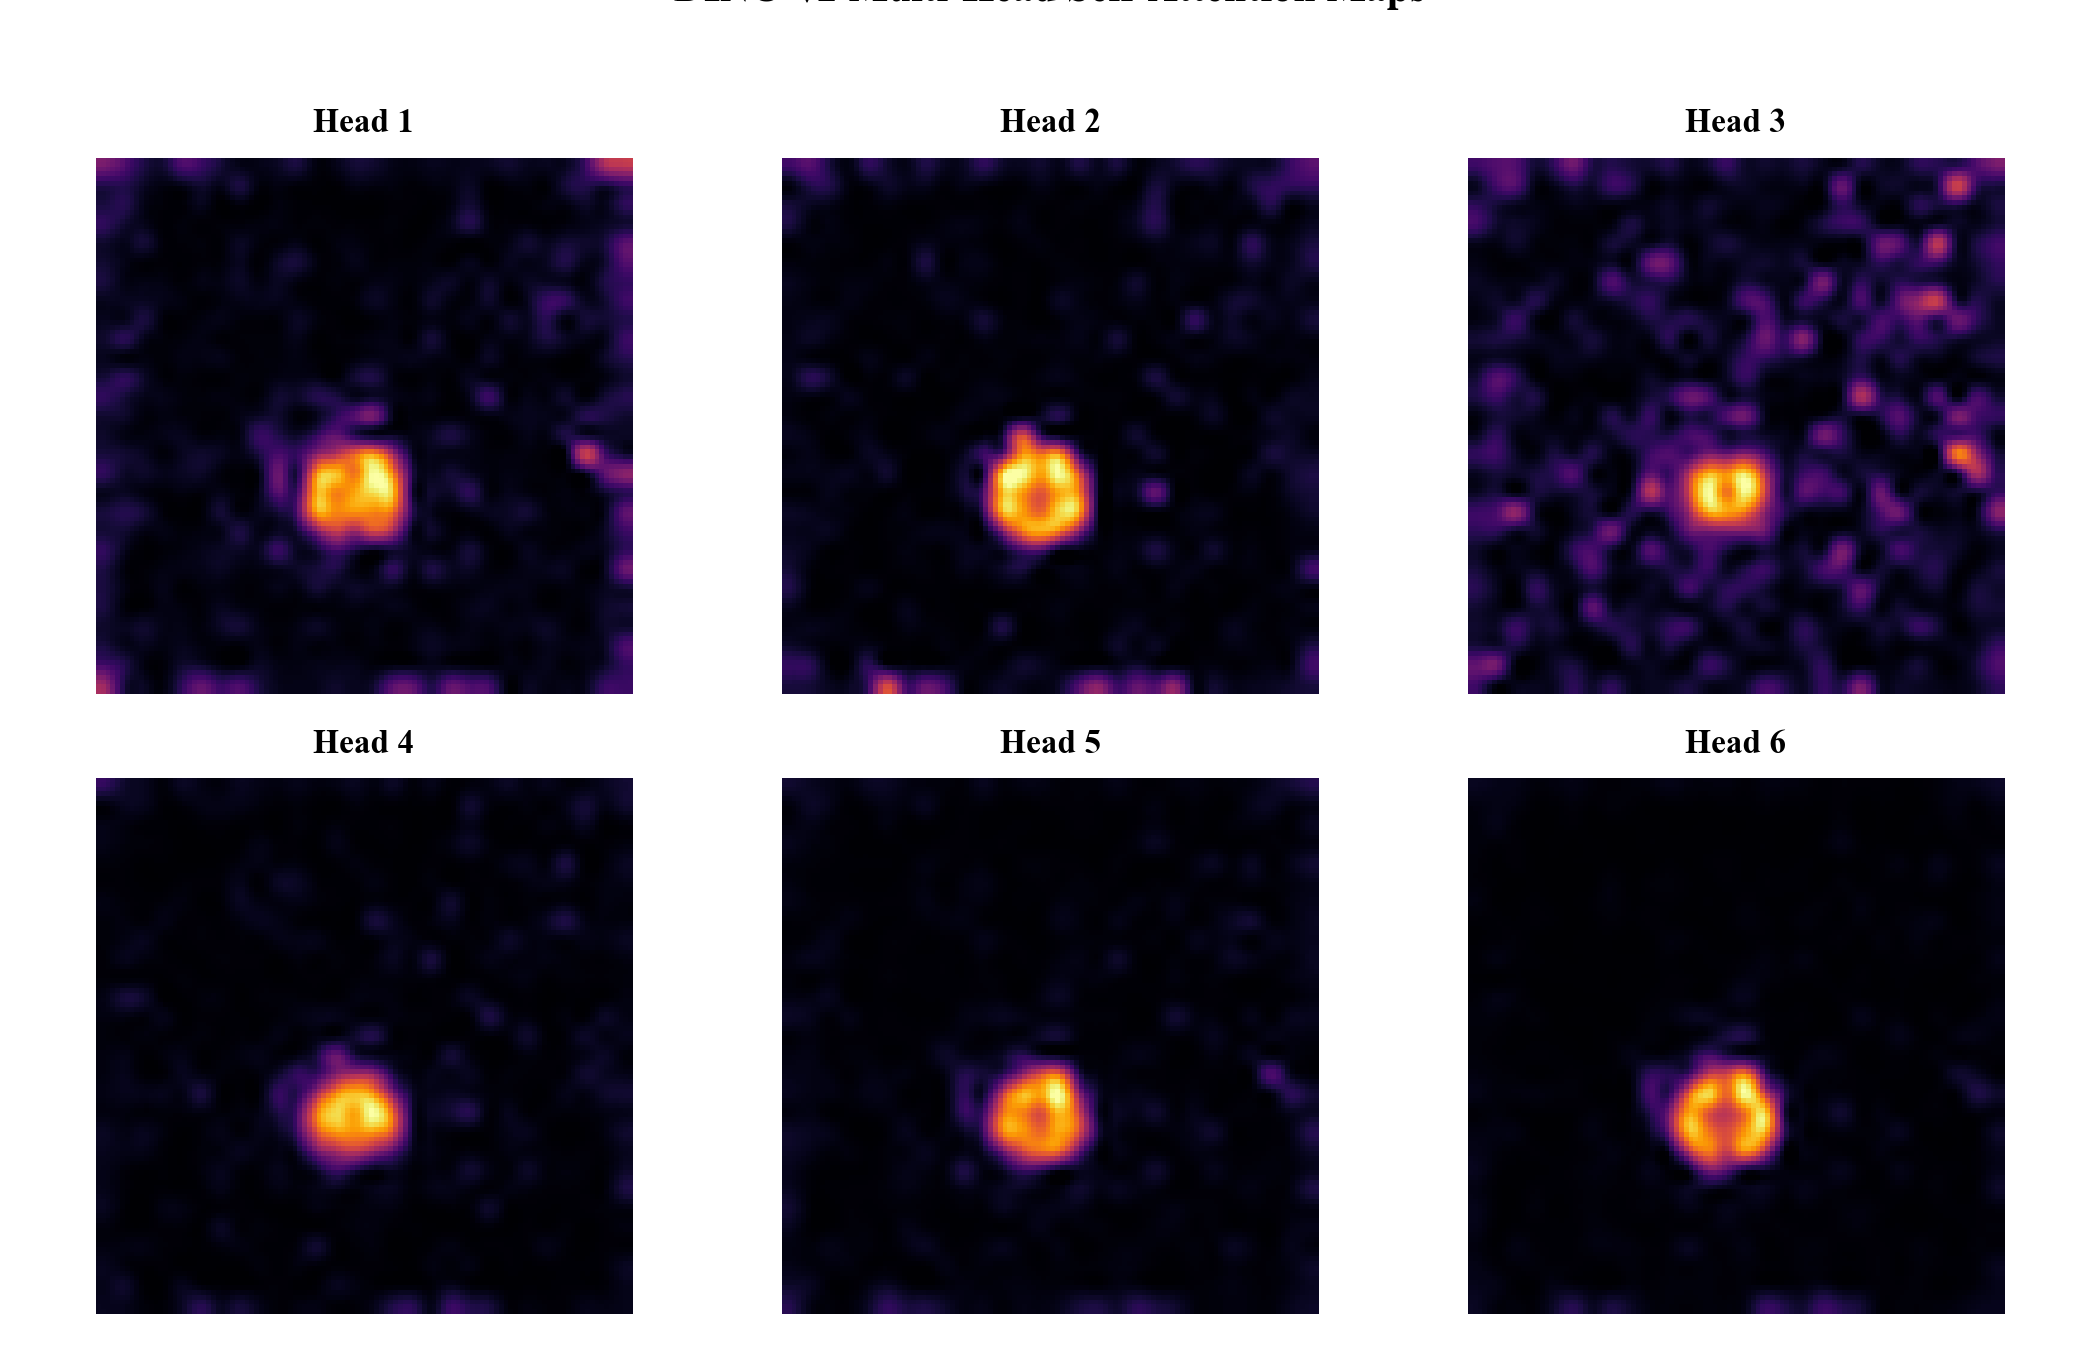
\includegraphics[width=0.9\textwidth]{Figures/attention_heads.png}
\caption{The six DINO self-attention heads for a defective fabric sample. Individual heads emphasize distinct thread orientations and texture patterns, and their combination highlights the anomalous region.}
\label{fig:attn}
\end{figure}

\subsection{ViT Autoencoder: Reconstruction Error}
The Vision Transformer Autoencoder learns to reconstruct defect-free fabric through a transformer encoder--decoder bottleneck, minimizing mean-squared reconstruction error. Anomalous regions, absent from the learned manifold, reconstruct poorly and produce high error, giving a third, orthogonal detection signal.

\section{Two Engineering Principles}

\subsection{Preprocessing Parity}
Because memory-bank and reconstruction detectors measure distance from a stored notion of ``normal,'' any image transform applied before inference becomes part of that definition. If the transform used at inference differs from the one used when the models were fitted, even normal cloth is scored as anomalous. Enforcing byte-level parity between the fit-time and inference-time preprocessing is thus a correctness requirement, not a tuning choice.

\subsection{Score Calibration}
The three detectors emit scores on incomparable scales (Euclidean distance in different feature spaces versus per-pixel reconstruction error). Standardizing each score against its own normal-data mean and standard deviation converts them to z-scores with a common ``standard deviations above normal'' meaning, so that a uniform average is meaningful and a single interpretable threshold suffices.

\section{Tools Used}

The system is implemented in Python with PyTorch~\cite{paszke2019pytorch} for model definition and GPU tensor operations, \texttt{timm} for the ViT backbones, and OpenCV and NumPy for image handling. Scikit-learn provides evaluation metrics. The production service uses FastAPI with a Uvicorn server for REST and WebSocket endpoints, and is containerized with Docker for GPU deployment. A React/Vite dashboard provides live visualization.

Together these fundamentals---the anomaly-detection paradigm, the shared ViT backbone, three complementary scoring mechanisms, and the parity and calibration principles---define the building blocks from which the system architecture in Chapter~3 is assembled.
